
%(BEGIN_QUESTION)
% Copyright 2007, Tony R. Kuphaldt, released under the Creative Commons Attribution License (v 1.0)
% This means you may do almost anything with this work of mine, so long as you give me proper credit

Shown here is the response of a process to a single step-change on the controller output (made with the controller in ``manual'' mode).  Based on your observations, determine the steady-state gain ($K$), dead time ($L_R$), and reaction rate ($R_R$):

$$\includegraphics[width=15.5cm]{i01656x01.eps}$$

$K$ = \underbar{\hskip 50pt} \hskip 50pt $L_R$ = \underbar{\hskip 50pt} \hskip 50pt $R_R$ = \underbar{\hskip 50pt}

\vskip 10pt

Suppose that this process were to be subjected to a larger step-change in output, say 25\% instead of 15\%.  What effect would this have had on the L$_{R}$ and R$_{R}$ calculations?

\vskip 10pt

Finally, calculate the time constant ($\tau$) of this process.

\underbar{file i01656}
%(END_QUESTION)





%(BEGIN_ANSWER)

$$\includegraphics[width=15.5cm]{i01656x02.eps}$$

\begin{itemize}
\item{}Steady-state gain ($K$) = 1.333
\vskip 5pt
\item{}Dead time ($L_R$) = 0.375 minutes
\vskip 5pt
\item{}Reaction rate ($R_R$) = 3.556\% / unit-minute
\end{itemize} 

\vskip 10pt

Note: the unit of ``unit-minute'' for reaction rate refers to reaction rate corrected for percentage of output step.  In other words, this is not the raw reaction rate figure, but rather the reaction rate per percent of output step.

\vskip 10pt

Ideally, there will be minimal effect on the apparent dead time ($L_R$) of the process, since such ``transport delays'' are usually unrelated to the manipulated variable.
 
The reaction rate ($R_R$) will also (ideally) remain constant.  Although the slope of the tangent line to the point of inflection on the PV curve will be steeper, this increase in steepness should be proportional to the increase in output step-change, resulting in an $R_R$ figure that is the same as with a lesser output step-change.

Of course, if the process gain changes throughout the PV range, then the reaction rate ($R_R$) will be affected by an increase in output step-change.

\vskip 10pt

$\tau$ = 0.375 minutes (approximately)

%(END_ANSWER)





%(BEGIN_NOTES)

{\it Calculating process gain:}

$K$ = $\Delta$PV / $\Delta$Output

$K$ = 20\% / 15\%

$K$ = 1.3333
 
\vskip 10pt

{\it Calculating apparent dead time:}

$L_R$ = (3 horizontal divisions on plot)(7.5 seconds / division)

$L_R$ = 22.5 seconds

$L_R$ = 0.375 minutes
 
\vskip 10pt
 
{\it Calculating reaction rate:}

$R_R$ = $\Delta$PV / (Lag time)($\Delta$Output)

$R_R$ = 20\% / (0.375 min)(15\%)

$R_R$ = 3.556\% / unit-minute
 
\vskip 10pt
 
NOTE: Some references suggest to calculate the reaction rate ($R_R$) as shown: the slope of the tangent line in \% per minute, per unit of output change.  Others omit the percent of output change, leading to an $R_R$ figure in units of \% per minute, but they assume an output change of only 1\% (1 unit), or else they incorporate the $\Delta$Output figure in a later equation when $R_R$ is used to calculate ideal PID constants.  

The tangent line slope is meaningless unless referenced to a specified change in output, since different step-changes in the output signal will lead to different rates of PV change per minute.

\vskip 10pt


Time constant ($\tau$) may be calculated two different ways:
 
\vskip 10pt

$\tau$ = Time required for PV to change 63.2\% from starting to final value (from the time the PV first starts to change -- no need to draw a reaction rate tangent line).
 
\vskip 10pt

$\tau$ = Time required for reaction rate tangent line to span full $\Delta$PV.

\vskip 10pt

NOTE: these two methods often produce significantly different results.  When in doubt, the best method to use is the first one, measuring the 63.2\% point on the vertical scale and then counting horizontal units of time.

%INDEX% Control, PID tuning: step change (output) revealing process gain
%INDEX% Control, PID tuning: step change (output) revealing process dead time
%INDEX% Control, PID tuning: step change (output) revealing process reaction rate

%(END_NOTES)


